\chapter{Datensatz}\label{chap:dataset}
\section{Beschreibung}
Der Udacity Self Driving Car Dataset \cite{datasetSelfDrivingCar} ist eine umfangreiche Sammlung von Bildern, die von Kameras in Fahrzeugen aufgenommen wurden. Der Datensatz beinhaltet 15000 Samples mit einer Auflösung von $512x512$ Pixeln. Er besteht aus Bildern und die zugehörigen Annotationen, die Informationen über die enthaltenen Objekte in der Umgebung enthalten.

Die Bilder in dem Datensatz umfassen verschiedene Szenarien im Straßenverkehr. Darunter befinden sich Stadt- und Landstraßen. Die Bilder wurden bei unterschiedlichen Lichtbedingungen aufgenommen, um ein breite Vielfalt an Situationen in den Daten abzudecken. 


\section{Klassenaufteilung}
\begin{figure}
	\begin{subfigure}{0.5\textwidth}
		\centering
		\begin{tabular}{l|c|c}
			\hline
			Klassen & Anzahl & Index \\
			\hline
			\hline
			car & 64399 & 0 \\
			pedestrian & 10806 & 1 \\
			trafficLight-Red & 6870 & 2 \\
			trafficLight-Green & 5465 & 3 \\
			truck & 3623 & 4 \\
			trafficLight & 2568 & 5 \\
			biker & 1846 & 6 \\
			trafficLight-RedLeft & 1751 & 7 \\
			trafficLight-GreenLeft & 310 & 8 \\
			trafficLight-Yellow & 272 & 9 \\
			trafficLight-YellowLeft & 14 & 10 \\
			\hline
		\end{tabular}
		\caption{Klassenverteilung der rohen Daten als Tabelle}
		\label{tab:classDistributionRaw_graph}
	\end{subfigure}%
	\begin{subfigure}{0.5\textwidth}
	\centering
	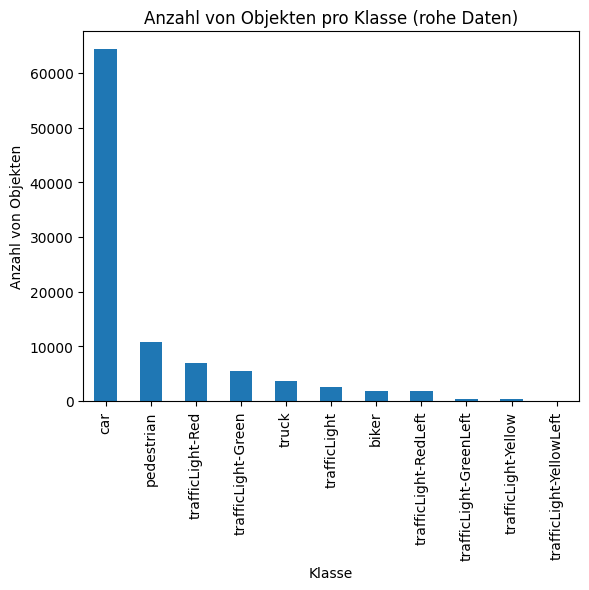
\includegraphics[width=\linewidth]{classDistribution_raw.png}
	\caption{Klassenverteilung der rohen Daten als Diagramm}
	\label{fig:classDistributionRaw_graph}
	\end{subfigure}%
	\caption{Klassenverteilung der rohen Daten}
	\label{fig:classDistributionRaw}
\end{figure}

\begin{figure}
	\begin{subfigure}{0.5\textwidth}
	\centering
	\begin{tabular}{l|c|c}
		\hline
		Klassen & Anzahl & Index \\
		\hline
		\hline
		car & 64399 & 0 \\
		pedestrian & 10806 & 1 \\
		trafficLight & 17250 & 2 \\
		truck & 3623 & 3 \\
		biker & 1846 & 4 \\
		\hline
	\end{tabular}
	\caption{Klassenverteilung der neuen Klassen als Tabelle}
	\label{tab:classDistributionNewClasses}
	\end{subfigure}
	\begin{subfigure}{0.5\textwidth}
		\centering
		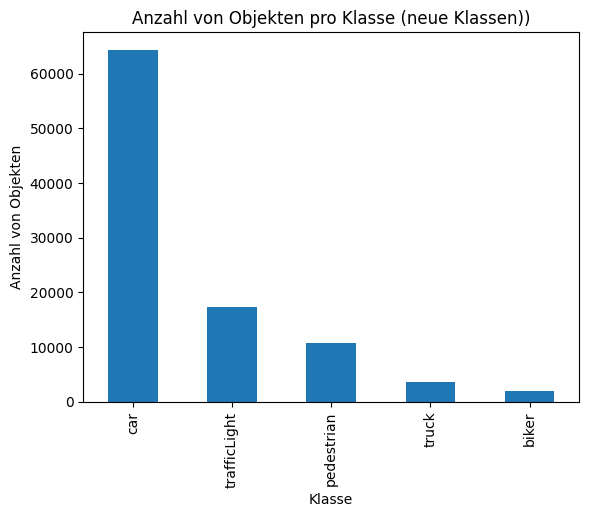
\includegraphics[width=\linewidth]{classDistribution_newClasses.png}
		\caption{Klassenverteilung der neuen Klassen als Diagramm}
		\label{fig:classDistributionNewClasses_graph}
	\end{subfigure}
	\caption{Klassenverteilung der neuen Klassen}
	\label{fig:classDistributionNewClasses}
\end{figure}

\begin{figure}
	\centering
		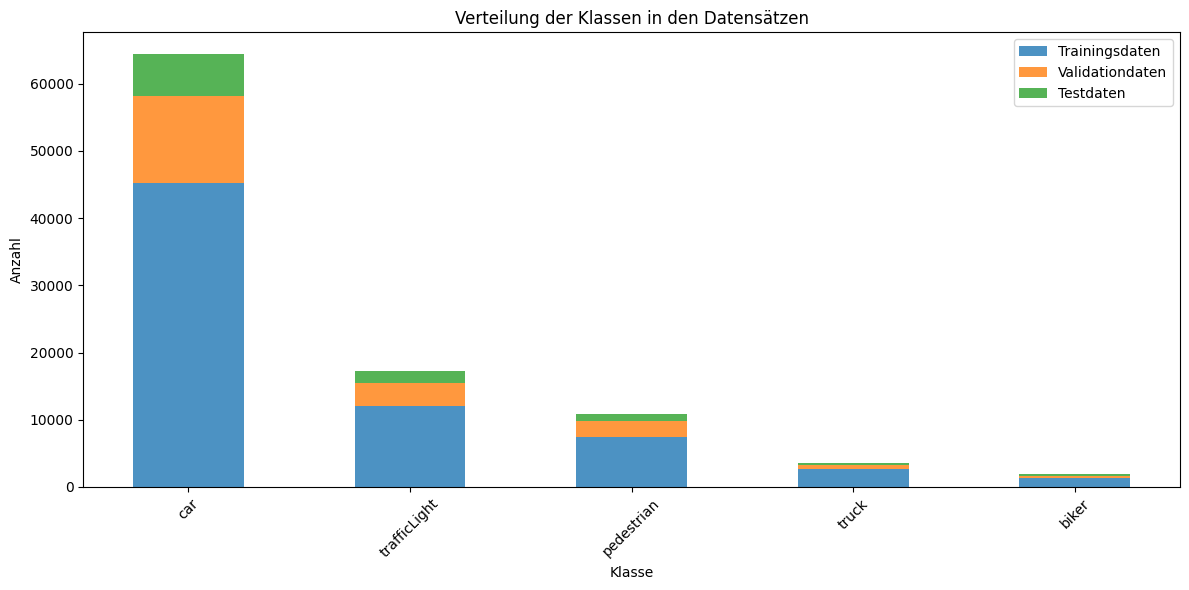
\includegraphics[width=\linewidth]{classDistribution_newClassesTrainValTest.png}
		\caption{Aufteilung in Trainings-, Validation- und Testdaten}
		\label{fig:datasetTrainValTestSplit}
\end{figure}


\section{Aufbau}
\subsection{Rohdaten}



\subsection{YOLOX}




\subsection{YOLOv8}




